\published{IEEE Geoscience and Remote Sensing Letters, 12, no. 10, 2150-2154, (2015)}

\title{De-aliased seismic data interpolation using seislet transform with low-frequency constraint}
\renewcommand{\thefootnote}{\fnsymbol{footnote}}

\author{Shuwei Gan\footnotemark[1], Shoudong Wang\footnotemark[1], Yangkang Chen\footnotemark[2], Yizhuo Zhang\footnotemark[3], Zhaoyu Jin\footnotemark[4]}
\address{
\footnotemark[1]
State Key Laboratory of Petroleum Resources and Prospecting \\
China University of Petroleum \\
Fuxue Road 18th\\
Beijing, China, 102200 \\
%331334826@qq.com
gsw19900128@126.com\\
\footnotemark[2] Jackson School of Geosciences\\
The University of Texas at Austin\\
University Station, Box X\\
Austin, TX 78713-8924, USA \\
Email: ykchen@utexas.edu\\
\footnotemark[3] Institut de Physique du Globe de Paris (IPGP)\\ 
1 Rue Jussieu\\
75005 Paris, France  \\
Email: yizhuozh@gmail.com\\
\footnotemark[3]School of Geosciences,
University of Edinburgh,
Edinburgh,UK, EH9 3JW,
Email: s1263999@sms.ed.ac.uk
}

\maketitle

\begin{abstract}
Interpolating regularly missing traces in seismic data is thought to be much harder than interpolating irregularly missing seismic traces, because many sparsity-based approaches can not be used due to the strong aliasing noise in the sparse domain. We propose to use seislet transform to perform a sparsity-based approach to interpolate highly under-sampled seismic data based on the classic projection onto convex sets (POCS) framework. Many numerical tests show that the local slope is the main factor that will affect the sparsity and anti-aliasing ability of seislet transform. By low-pass filtering the under-sampled seismic data with a very low bound frequency, we can get a precise dip estimation, which will make seislet transform capable for interpolating the aliased seismic data. In order to prepare the optimum local slope during iterations, we update the slope field every several iterations. We also use a percentile thresholding approach to better control the reconstruction performance. Both synthetic and field examples show better performance using the proposed approach than the traditional prediction based and the $F-K$ POCS based approaches.
\end{abstract}

%\begin{keywords}
%Seismic data interpolation, seislet transform, sparsity comparison, low-frequency constrained inversion, local slope
%\end{keywords}


\section{Introduction}
Due to different reasons, seismic data may have missing traces. Seismic data reconstruction is such a procedure to remove sampling artifacts, and to improve amplitude analysis, which are very important for subsequent processing steps including high-resolution processing, wave-equation migration, multiple suppression, amplitude-versus-offset (AVO) or amplitude-versus-azimuth (AVAZ) analysis, and time-lapse studies \cite{daniel2002,liubin2004,abma2005,juefu2010,mostafa2010,yangkang2015eage2}. In recent years, due to the development of compressive sensing framework, there are a lot of sparsity-based methods for interpolating irregularly sampled seismic data. However, for regularly missing traces, sparsity-based methods \cite{abma2006,chengbo2012,yangkang2014halfthr} can not obtain satisfying results because of the strong aliasing noise in the transform domain. Instead, the prediction-based approaches \cite{spitz1991,mostafa2007} are still the best approaches for interpolating regularly missing traces. 

In this paper, we propose to use seislet transform to perform a sparsity-based reconstruction, based on the well-established projection onto convex sets (POCS) framework \cite{abma2006}. Many numerical studies show that the local slope is the main factor affecting the sparsity and anti-aliasing ability of the seislet transform. Even though with the original aliased data, we can not obtain precise dip estimation, we can use low-pass filtered data (below 15 Hz) to estimate local slope in order to construct the seislet transform of the full-band seismic data and perform thresholding. Synthetic data and field data examples show nearly perfect results using the proposed approach. The traditional prediction based approach and the $F-K$ based POCS approach are both compared with the proposed approach and are demonstrated to be less effective.

\section{Methods}
\subsection{Projection onto convex sets (POCS)}
The principal problem of seismic data reconstruction is to solve the under-determined inversion problem:
\begin{equation}
\label{eq:acq}
\mathbf{Fm}=\mathbf{d},
\end{equation}
where $\mathbf{m}$ is the well-sampled seismic data, $\mathbf{F}$ denotes the sampling operator, and $\mathbf{d}$ denotes the observed data \cite{yangkang2014halfthr}. Because of the missing traces, the operator $\mathbf{F}$ is highly singular and thus make equation \ref{eq:acq} highly under-determined.

There have existed many different algorithms for solving equation \ref{eq:acq} by adding different constraints. The POCS algorithm \cite{abma2006} is one of the most widely used methods to interpolate seismic data with irregularly missing traces, and has the following iterative expression:
\begin{equation} 
\label{eq:pocs}
\mathbf{m}_{n+1}=\mathbf{d}+(\mathbf{I}-\mathbf{F})\mathbf{A}^{-1}\mathbf{T}\mathbf{A}[\mathbf{m}_n],
\end{equation}
where $\mathbf{m}_n$ denotes the reconstructed data after $n$th iteration, $\mathbf{A}$ and $\mathbf{A}^{-1}$ are the forward and inverse sparsity-promoting transforms, $\mathbf{I}$ is an identity matrix and $\mathbf{T}$ is a thresholding operator. However, for regularly missing traces, POCS can not obtain satisfying results because of the strong aliasing noise in the sparse domain

\subsection{Seislet transform}
The construction of seislet transform \cite{seislet} follows the basics of the second-generation wavelet transform. The forward transform starts with the finest scale (the original sampling) and goes to the coarsest scale. The inverse transform starts with the coarsest scale and goes back to the finest scale \cite{yangkang20142}. The forward and inverse seislet transforms can be
expressed as:
\begin{equation}
\label{eq:one}
\mathbf{r}=\mathbf{o}-\mathbf{P\left[e\right]},
\end{equation}
\begin{equation}
\label{eq:two}
\mathbf{c}=\mathbf{e}+\mathbf{U\left[r\right]},
\end{equation}
\begin{equation}
\label{eq:three}
\mathbf{e}=\mathbf{c}-\mathbf{U\left[r\right]},
\end{equation}
\begin{equation}
\label{eq:four}
\mathbf{o}=\mathbf{r}+\mathbf{P\left[e\right]},
\end{equation}
where $\mathbf{P}$ is the prediction operator, $\mathbf{U}$ is the updating operator. $\mathbf{r}$ denotes the difference between true odd trace and predicted odd trace (from even trace), $\mathbf{c}$ denotes a coarse approximation of the data. At the start of the forward transform, e and o correspond to the even and odd traces of the data domain. At the start of the inverse transform, $\mathbf{c}$ and $\mathbf{r}$ will have just one
trace of the coarsest scale of the seislet domain. The seislet transform differs from the wavelet transform in that the prediction and updating operators utilize the local slope of seismic profiles to predict and update the even and odd traces. The above prediction and update operators can be defined as follows:
\begin{equation}
\label{eq:five}
\mathbf{P}\left[\mathbf{e}\right]_k=\left(\mathbf{P}^{(+)}_k\left[\mathbf{e}_{k-1}\right]+\mathbf{P}^{(-)}_k\left[\mathbf{e}_k\right]\right)/2,
\end{equation}
\begin{equation}
\label{eq:six}
\mathbf{U}\left[\mathbf{r}\right]_k=\left(\mathbf{P}^{(+)}_k\left[\mathbf{r}_{k-1}\right]+\mathbf{P}^{(-)}_k\left[\mathbf{r}_k\right]\right)/4,
\end{equation}
where $\mathbf{P}^{(+)}_k$ and $\mathbf{P}^{(-)}_k$ are operators that predict a trace from its left and right neighbors, correspondingly, by shifting seismic events according to their local slopes.
The local slope can be calculated using a robust algorithm as introduced in \cite{fomel2002pwd}.

\begin{figure}[htb!]
  \centering
    \subfloat[]{\includegraphics[width=0.36\columnwidth]{coef/Fig/hyper-fk}
    \label{fig:hyper-fk}}
    \subfloat[]{\includegraphics[width=0.36\columnwidth]{coef/Fig/hyper-dwt}
    \label{fig:hyper-dwt}}
    \subfloat[]{\includegraphics[width=0.36\columnwidth]{coef/Fig/hyper-seiss}
    \label{fig:hyper-seiss}}
    \subfloat[]{\includegraphics[width=0.36\columnwidth]{coef/Fig/hyper-curv-img}
    \label{fig:hyper-curv-img}}    
	\caption{Comparison among different sparsity-promoting transforms based on the synthetic example shown in Figure \ref{fig:hyper}. (a) 2-D Fourier transform domain. (b) 2-D Wavelet transform domain. (c) 2-D Seislet transform domain. (d) 2-D Curvelet transform domain.}
   \label{fig:hyper-fk,hyper-dwt,hyper-seis,hyper-curv-img}
\end{figure}

\begin{figure}[htb!]
  \centering
    \includegraphics[width=0.5\columnwidth]{coef/Fig/hyper-c}
	\caption{Coefficients decaying diagram of different sparsity-promoting transforms.}
   \label{fig:hyper-c}
\end{figure}

\begin{figure}[htb!]
  \centering
    \subfloat[]{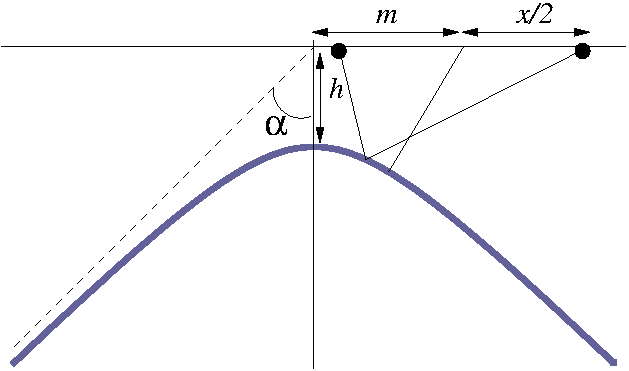
\includegraphics[width=0.36\columnwidth]{synth/Fig/hyper}
    \label{fig:hyper}}
  \subfloat[]{\includegraphics[width=0.36\columnwidth]{synth/Fig/hyper-zero}
    \label{fig:hyper-zero}}
  \subfloat[]{\includegraphics[width=0.36\columnwidth]{synth/Fig/fk-hyper}
    \label{fig:fk-hyper}}
  \subfloat[]{\includegraphics[width=0.36\columnwidth]{synth/Fig/fk-hyper-zero}
    \label{fig:fk-hyper-zero}}
	\caption{(a) Original synthetic data. (b) Decimated data (50\% traces regularly removed). (c) $F-K$ spectrum of original synthetic data. (d)  $F-K$ spectrum of decimated data }
   \label{fig:hyper,hyper-zero,fk-hyper,fk-hyper-zero}
\end{figure}

\begin{figure}[htb!]
  \centering
    \subfloat[]{\includegraphics[width=0.36\columnwidth]{synth/Fig/hyper-seis}
    \label{fig:hyper-seis}}
    \subfloat[]{\includegraphics[width=0.36\columnwidth]{synth/Fig/hyper-fx}
    \label{fig:hyper-fx}}
  \subfloat[]{\includegraphics[width=0.36\columnwidth]{synth/Fig/fk-hyper-seis}
    \label{fig:fk-hyper-seis}}
  \subfloat[]{\includegraphics[width=0.36\columnwidth]{synth/Fig/fk-hyper-fx}
    \label{fig:fk-hyper-fx}}
	\caption{(a) Reconstructed data using the proposed approach. (b) Reconstructed data using Spitz's approach. (c)  $F-K$ spectrum of reconstructed data using the proposed approach. (d)  $F-K$ spectrum of reconstructed data using Spitz's approach. }
   \label{fig:hyper-seiss,hyper-fx,fk-hyper-seis,fk-hyper-fx}
\end{figure}


\begin{figure}[htb!]
  \centering
    \subfloat[]{\includegraphics[width=0.36\columnwidth]{synth/Fig/hyper-seis-dif}
    \label{fig:hyper-seis-dif}}
    \subfloat[]{\includegraphics[width=0.36\columnwidth]{synth/Fig/hyper-fx-dif}
    \label{fig:hyper-fx-dif}}
	\caption{(a) Reconstruction error using the proposed approach. (b) Reconstruction error using the Spitz's approach.}
   \label{fig:hyper-seis-dif,hyper-fx-dif}
\end{figure}


\begin{figure}[htb!]
  \centering
    \subfloat[]{\includegraphics[width=0.36\columnwidth]{synth/Fig/dip}
    \label{fig:dip}}
  \subfloat[]{\includegraphics[width=0.36\columnwidth]{synth/Fig/dip-pocs66}
    \label{fig:dip1}}
    \subfloat[]{\includegraphics[width=0.36\columnwidth]{synth30Hz/Fig/dip-pocs66}
    \label{fig:dip2}}
	\caption{(a) Accurate dip estimation. (b) Final dip estimation using 15 Hz low-pass filtering. (c) Final dip estimation using 30 Hz low-pass filtering. Note the aliased dip in (c).}
   \label{fig:dip,dip1,dip2}
\end{figure}

\begin{figure}[htb!]
  \centering
    \includegraphics[width=0.5\columnwidth]{synth/Fig/snrs-pocs}
	\caption{Convergence diagram of the first example using the proposed approach.}
   \label{fig:snrs-pocs}
\end{figure}

\subsection{Comparison of sparsity-promoting transforms}
The well-known existing sparsity-promoting transforms in the exploration geophysics field include the Fourier\cite{chandrasekharan1949}, wavelet transform\cite{akansu2010}, and curvelet transform \cite{candes20061}. 

In order to effectively compare the sparseness of different transforms, we first select an input dataset (here, we use the synthetic example shown in Figure \ref{fig:hyper} as the input dataset). Then we transform the input data into sparse transform domain using different sparse transforms. Figure \ref{fig:hyper-fk,hyper-dwt,hyper-seis,hyper-curv-img} shows different transformed domains for the input data. The 2-D Fourier transform in this case means the $f-k$ transform. The 2-D wavelet transform means implementing the 1-D wavelet transform along the temporal direction first and along the spatial direction second. The 2-D seislet transform means implementing the seislet transform along the spatial direction first and 1-D seislet transform along the temporal direction second. The 2-D curvelet transform refers to the 2-D wedge wrapping based fast discrete curvelet transform \cite{candes20061}. Next we sort the coefficients in the transform domains into decaying 1-D vectors according to the coefficient amplitude and scale the 1-D vectors. Finally we plot the decaying coefficients with respect to the sequence number for all the transforms in one plot. Figure \ref{fig:hyper-c} shows a comparison between the decay of sorted coefficients in the 2-D Fourier transform, 2-D wavelet transform, 2-D seislet transform and 2-D curvelet transform domains. Our experiments show that the seislet coefficients decay significantly faster than coefficients of the other transforms, which indicates a more compact structure of the seislet domain. Thus, our POCS based interpolation approach is preferred to use the 2-D seislet transform domain as the sparsity-promoting transform. Although the sparsity comparison is based on the well-sampled data, the same conclusion can be extended to the under-sampled case. It is worth to be mentioned that most sparse transforms (in their original form) including the four mentioned transforms can not obtain acceptable reconstruction results for under-sampled data with regularly missing traces.


\subsection{De-aliased interpolation by low-frequency constrained local slope estimation}
It can be demonstrated by tests that the slope estimation is the main factor affecting the sparsity and anti-aliasing ability of the seislet transform. Thus, we can first filter the data using a simple low-pass filter with a very low bound frequency. The bound frequency can be different for different datasets, but is generally below 15 Hz. When interpolating the regularly missing traces using a POCS algorithm, there are three key factors that will affect the final reconstructed results: (1) Slope estimation. (2) Threshold value in the seislet transform. (3) Number of iterations. We re-estimate the dip about every 5 POCS iterations using the low-pass filtered data. In order to set the optimum threshold, we use a percentile strategy, assuming that a certain percentage of coefficients can represent the data. In order to obtain a very good reconstruction, the number of iterations should be relatively large (about 150 iterations). The main computational cost of the proposed approach lays on the forward and inverse seislet transforms \cite{seislet,yangkang20142}. The seislet transform can be more expensive than the fast Fourier transform and the digital wavelet transform, but still has an $O(N)$ cost and is still efficient in practice.

\section{Examples}
The first synthetic example is shown in Figures \ref{fig:hyper,hyper-zero,fk-hyper,fk-hyper-zero}, \ref{fig:hyper-seiss,hyper-fx,fk-hyper-seis,fk-hyper-fx}, \ref{fig:hyper-seis-dif,hyper-fx-dif}, \ref{fig:dip,dip1,dip2} and \ref{fig:snrs-pocs}. Figure \ref{fig:hyper} shows the original well-sampled data. By regularly removing 50 \% traces, we simulate the under-sampled data and show it in Figure \ref{fig:hyper-zero}. After using the proposed approach, we obtain a perfect reconstructed data as shown in Figure \ref{fig:hyper-seis}. The dip estimation is applied on the low-frequency data using 15 Hz low-pass filtering. During each iteration, we preserve 8\% coefficients. In order to numerically compare the denoising performances of different approaches,  we utilize the signal-to-noise ratio (SNR) \cite{yangkang2015}:
\begin{equation}
\label{eq:snr}
SNR_n=10\log_{10}\frac{\Arrowvert \mathbf{m} \Arrowvert_2^2}{\Arrowvert \mathbf{m}-\mathbf{m}_n\Arrowvert_2^2},
\end{equation}
where $\mathbf{m}$ is the original complete data and $\mathbf{m}_n$ is denotes the reconstructed data after $n$th iteration.
After 200 iterations, we obtain a well-reconstructed data with a high SNR: 28.02 dB. Figure \ref{fig:snrs-pocs} shows the convergence diagram in terms of SNR using the proposed approach. It is clear that the percentile thresholding strategy can help obtain a converged result with a high SNR. Figures \ref{fig:fk-hyper} and \ref{fig:fk-hyper-zero} show the $F-K$ spectrum of the original data and decimated data. It is obvious that the removed traces cause strong spatial aliasing in the spectrum (Figure \ref{fig:fk-hyper-zero}). We also use the traditional $F-X$ prediction based approach \cite{spitz1991} to interpolate the decimated data and show the result in Figure \ref{fig:hyper-fx}. The performance of $F-X$ prediction method also obtains a good recovery of the missing traces. However, when compared in the $F-K$ domain (Figures \ref{fig:fk-hyper-seis} and \ref{fig:fk-hyper-fx}), the proposed approach clearly does a better job because there is still some aliasing noise left in the spectrum from $F-X$ prediction method. It can be further confirmed from the interpolation error sections, as shown in Figure \ref{fig:hyper-seis-dif,hyper-fx-dif}. $F-X$ prediction method causes noticeable estimation error while the proposed approach causes nearly zero error. 

As we can see, the spectrum of the reconstructed data using the proposed approach is exactly the same as the original data. If we use a filter with a somewhat higher low-pass frequency, we will obtain a much worse reconstructed result, because of the severe aliasing problem. Figure \ref{fig:dip} shows the precise dip estimation from the original data. Figure \ref{fig:dip1} shows the final dip estimation using 15 Hz low-pass filtering. The final dip estimation using 30 Hz low-pass filtering shows incorrect dips around 0.75 s at trace 250 (Figure \ref{fig:dip2}). 

The second synthetic example is a linear-event example to test the performance of the proposed approach on post-stack data. The original data is shown in Figure \ref{fig:linear}. We also remove 50\% traces regularly. In this example, we compare the proposed approach with the $F-K$ based POCS approach. The reconstructed results using the proposed approach and the $F-K$ based POCS approach are shown in Figures \ref{fig:linear-seis} and \ref{fig:linear-fft}, respectively. It is obvious that the proposed can still obtain a perfect performance, while the $F-K$ based POCS approach cannot obtain any improvement because of the strong aliasing noise in the $F-K$ domain. This test confirms the fact that $F-K$ based POCS approach should not be used to interpolate regularly missing traces \cite{spitz1991,mostafa2007,mostafa2010}. In this example, we use 100 iterations to obtain the reconstructed results of both seislet and Fourier transforms. The final SNR of the proposed approach reaches 22.47 dB, and the SNR of the $F-K$ based POCS approach stays unchanged: 3.007 dB. The slightly worse performance of the proposed approach on this example than the first example is because the crossing seismic events cause some errors when estimating the local slope, which affect the final performance a bit.  

\begin{figure}[htb!]
  \centering
    \subfloat[]{\includegraphics[width=0.36\columnwidth]{linear/Fig/linear}
    \label{fig:linear}}
    \subfloat[]{\includegraphics[width=0.36\columnwidth]{linear/Fig/linear-zero}
    \label{fig:linear-zero}}\\
    \subfloat[]{\includegraphics[width=0.36\columnwidth]{linear/Fig/linear-seis}
    \label{fig:linear-seis}}
    \subfloat[]{\includegraphics[width=0.36\columnwidth]{linear/Fig/linear-fft}
    \label{fig:linear-fft}}    
	\caption{Second synthetic example test. (a) Original synthetic data. (b) Decimated data (50\% traces regularly removed). (c) Reconstructed data using the proposed approach. (d) Reconstructed data using $F-K$ based POCS approach. Note that the $F-K$ based POCS approach cannot obtain any improvement because of the aliasing noise caused by the regularly missing traces.}
   \label{fig:linear,linear-zero,linear-seis,linear-fft}
\end{figure}

The field data example is a highly under-sampled common shot gather, as shown in Figure \ref{fig:field}. By manually adding zero traces between two neighbor traces, we obtain the zero-padded data, as shown in Figure \ref{fig:field-zero}. After interpolation, a much better sampled data can be obtained, as shown in Figure \ref{fig:field-seis}. In this example, we estimate the local slope using 5 Hz low-pass filtering. The corresponding $F-K$ spectrum are shown in Figures \ref{fig:fk-field}, \ref{fig:fk-field-zero} and \ref{fig:fk-field-seis}, respectively. For many real seismic data, we might have difficulties to get the low-frequency information because of the low SNR at low frequencies. Thus, the proposed approach set a relatively high demand for data quality. Fortunately, we only require the low-frequency data for slope estimation and the appropriate frequency range varies from 5 Hz to 20 Hz for different datasets, which is not a problem for most field dataset.

\begin{figure}[htb!]
  \centering
    \subfloat[]{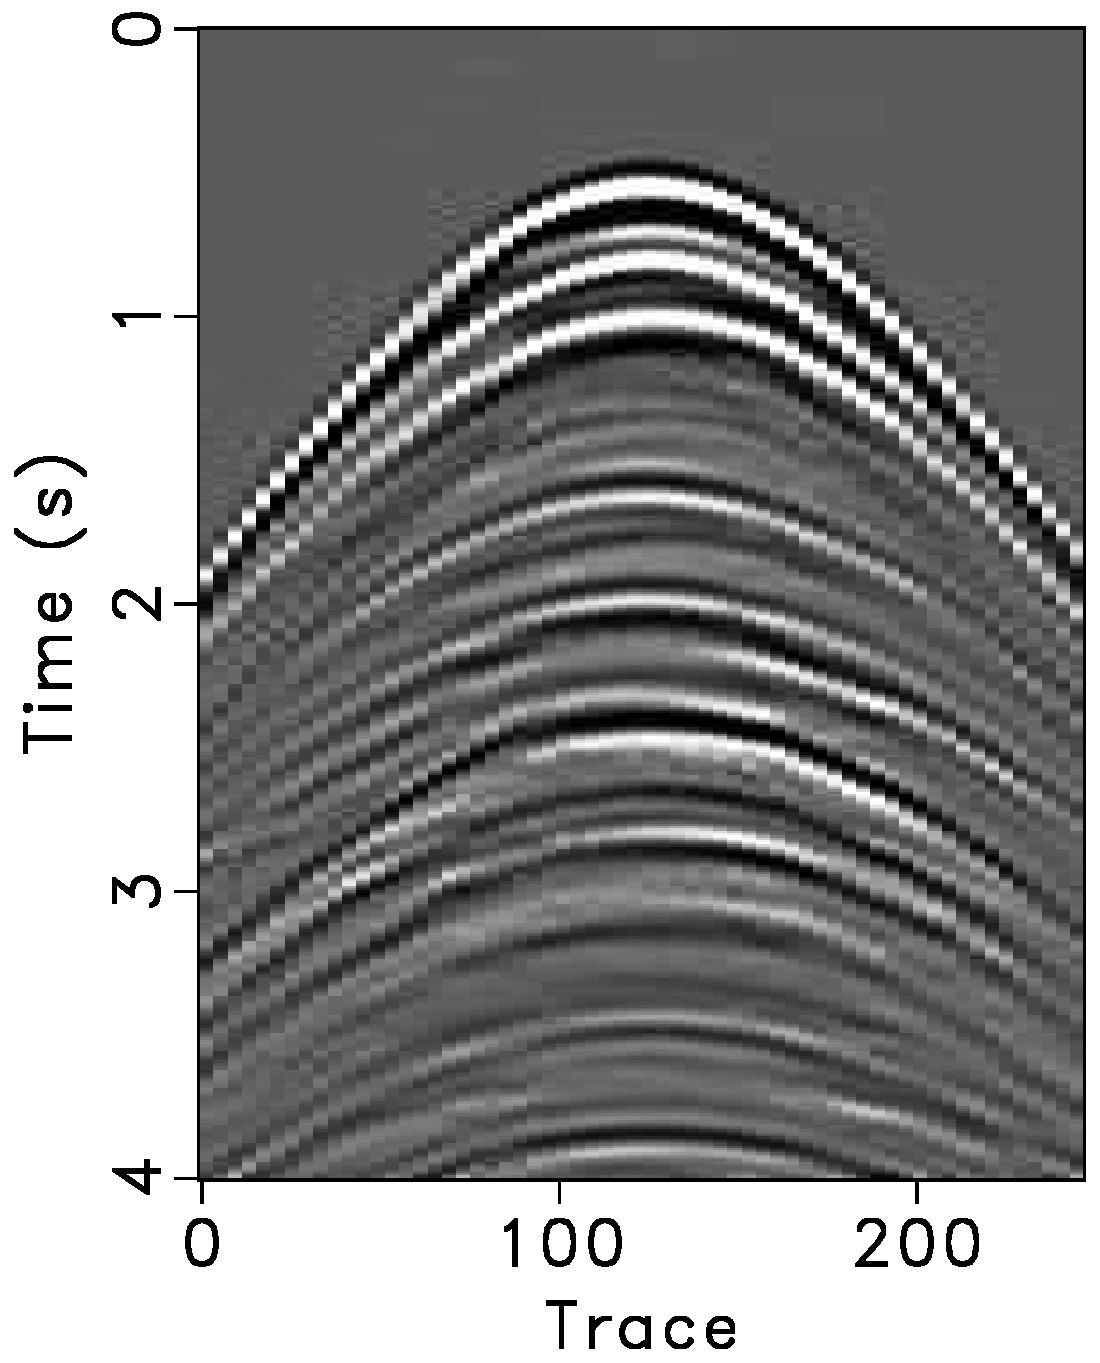
\includegraphics[width=0.29\columnwidth]{field/Fig/field}
    \label{fig:field}}
  \subfloat[]{\includegraphics[width=0.29\columnwidth]{field/Fig/field-zero}
    \label{fig:field-zero}}
    \subfloat[]{\includegraphics[width=0.29\columnwidth]{field/Fig/field-seis}
    \label{fig:field-seis}}\\
  \subfloat[]{\includegraphics[width=0.29\columnwidth]{field/Fig/fk-field}
    \label{fig:fk-field}}
  \subfloat[]{\includegraphics[width=0.29\columnwidth]{field/Fig/fk-field-zero}
    \label{fig:fk-field-zero}}
  \subfloat[]{\includegraphics[width=0.29\columnwidth]{field/Fig/fk-field-seis}
    \label{fig:fk-field-seis}}
	\caption{(a) Original field data. (b) Zero-padded field data. (c) Interpolated field data. (d) $F-K$ spectrum of original field data. (e) $F-K$ spectrum of zero-padded field data. (f) $F-K$ spectrum of interpolated field data.}
   \label{fig:field,field-zero,field-seis,fk-field,fk-field-zero,fk-field-seis}
\end{figure}

\section{Conclusion}
In this paper, we propose to use seislet domain percentile thresholding to iteratively reconstruct the regularly missing seismic traces based on the well-established POCS framework. Numerical tests show that the local slope is the main factor affecting the sparsity and anti-aliasing ability of seislet transform. %In order to provide the optimum slope estimation,
We update the local slope every several iterations and use low-frequency constrained data to prepare the local slope. We use both synthetic and field data examples to show nearly perfect reconstruction results using the proposed approach for reconstructing regularly missing traces. However, the $F-K$ based POCS approach cannot interpolate the irregularly missing traces because of the strong aliasing noise in the $F-K$ domain. The performance of the proposed approach is better than the commonly used $F-X$ prediction based interpolation approach. 
 
\section{Acknowledgements}
We would like to thank the associated editor Luis Gomez and two anonymous reviewers for constructive suggestions on the manuscript. This research is supported by the National Natural Science Foundation of China (Grant No.41274137), the National Science and Technology of Major Projects of China (Grant No. 2011ZX05019-006), and National Engineering Laboratory of Offshore Oil Exploration.

\bibliographystyle{seg}
\bibliography{dealiase}
